\documentclass[a4paper, twoside]{article}
\usepackage{geometry}
\usepackage{sidenotes}
\usepackage{marginfix}
\usepackage[T1]{fontenc}
% \usepackage{newtx}
\usepackage[scaled]{helvet}
\renewcommand{\familydefault}{\sfdefault}
\usepackage[scale]{plex-mono}
\usepackage{sidenotes}

\usepackage{listings}
\usepackage[svgnames]{xcolor}
\usepackage[T1]{fontenc}

% Style for code listings.
\lstdefinestyle{mystyle}{
    % backgroundcolor=\color{MintCream},
    commentstyle=\color{BlueViolet},
    keywordstyle=\color{magenta},
    frame=single,
    % numberstyle=\ttfamily\color{Gray},
    stringstyle=\color{DarkGreen},
    basicstyle=\ttfamily\small,
    showstringspaces=false,
    rulecolor=\color{Gray},
    breaklines=true,
    numbers=left,
    showstringspaces=false,
    % linewidth=340pt,
    % numbersep=1pt,
}

\geometry{
    paperwidth=210mm,
    paperheight=297mm,
    left=42pt,
    top=72pt,
    textwidth=340pt,
    marginparsep=20pt,
    marginparwidth=160pt,
    textheight=650pt,
    footskip=40pt,
}

\lstset{style=mystyle}
\usepackage{graphicx}

\newcommand{\pubstyle}{\texttt{pub\textunderscore style}}

\title{Making figures with \pubstyle}
\author{Abdullah Mustafa}
\date{June 13, 2026}

\begin{document}
\maketitle

I got tired of looking at horrible matplotlib fonts, so I wrote \pubstyle.

\lstinputlisting[language=Python]{simplest.py}
\begin{marginfigure}
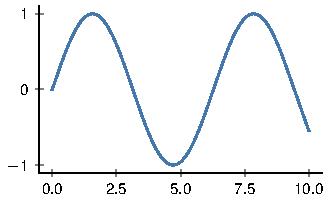
\includegraphics{simplest.pdf}
\end{marginfigure}

\lstinputlisting[language=Python]{laserAtThreshold.py}
That gets you this figure.
\begin{marginfigure}
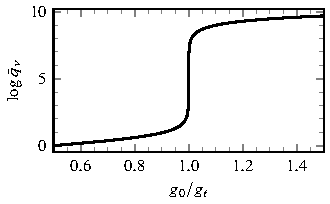
\includegraphics{laserAtThreshold.pdf}
\end{marginfigure}

That gets you this figure.
\begin{figure}
    \centering
    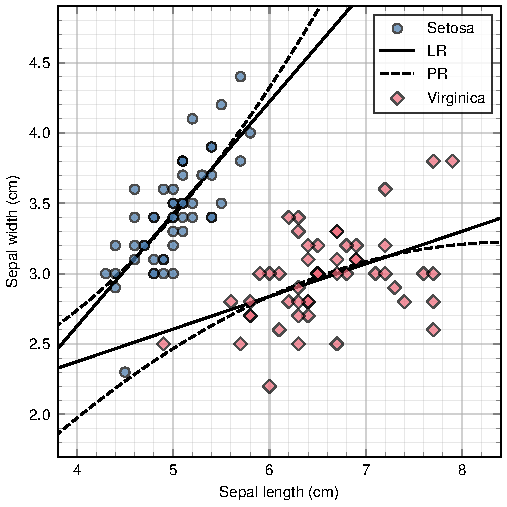
\includegraphics{regresfigure.pdf}
\end{figure}
\lstinputlisting[language=Python]{regresfigure.py}


\end{document}